\documentclass[a4paper, 10pt]{article}
\usepackage[utf8]{inputenc} % Change according your file encoding
\usepackage{graphicx}
\usepackage{url}
\usepackage{amsmath}
\usepackage{mathtools}
\usepackage{mathrsfs}
\usepackage{amsfonts}
\usepackage{bbm}
\usepackage{amsthm}
\usepackage{amssymb}
\usepackage{fancyhdr}
\usepackage{setspace}
\usepackage{tabularx}
\usepackage{tikz}
\usetikzlibrary{arrows,positioning}
\usepackage[a4paper, left=2cm, right=2cm, top=2.5cm, bottom=2cm]{geometry}

\pagestyle{fancy}
\fancyhf{}
\rhead{Tuesday, December 10th}
\lhead{Víctor Mart\'in, Pablo Oviedo, and Carlos Segarra - DAG: Sheet 1}
\cfoot{\thepage}

\newtheorem{obs}{Observation}
\newtheorem{theorem}{Theorem}
\newtheorem*{theoremstar}{Theorem}

\theoremstyle{definition} % amsthm only
\newtheorem{definition}{Definition}

%\newtheorem{def}{Definition}

\newcommand{\espai}{\vspace{3mm}}
\newcommand{\I}{\mathscr{I}}
\newcommand{\B}{\mathscr{B}}
\newcommand{\C}{\mathscr{C}}
\newcommand{\F}{\mathscr{F}}

\begin{document}
\onehalfspacing
\tikzstyle{vertice}=[circle, draw, fill=black!50, inner sep = 0pt, minimum width=4pt]

\textbf{\Large Discrete and Algorithmic Geometry: Sheet 1}

\vspace{20pt}

\textbf{\textit{(1) Let $M$ be a matroid on the ground set $[n] = \lbrace 1, 2, \dots, n \rbrace$ with family of independent sets $\lbrace I : I \in \mathcal{I}\rbrace$:}}

\vspace{3pt}

\hspace{5pt} \textbf{\textit{(a) Contraction in $M$ as defined in class agrees with the notion of contraction in graphs.}}

\vspace{3pt}

Let $G = (V, E)$ be a simple graph (no loops, no multiedges). Let $M = (E, \mathcal I)$ be a matroid, where $\mathcal I \subset \mathcal P(E)$, the family of independent sets of the matroid, is the set of acyclic subgraphs of $G$ (considering only their edges).

Let $e \in E$, and consider $I \in \mathcal I$ such that $I = \{e_0, e_1, \ldots e_r\}$, and $e \in I$ (let us assume WLOG $e = e_0$). Now, $I/e = \{e_1, \ldots, e_r\}$ is an acyclic subgraph of $G/e$, meaning $I'$ is an independent set of $M/e$.

Similarly, if $I' = \{e_1, \ldots, e_r\} \in \mathcal I(M/e)$ is an acyclic subgraph of $G/e$, $I = I' \cup \{e\}$ is an acyclic subgraph of $G$, meaning $I$ is an independent set of $M$.


\hspace{5pt} \textbf{\textit{(b) Contraction in $M$ as defined in class agrees with $M / S \coloneqq (M^\star \backslash S)^\star$ for a subset $S \subset [n]$.}}

\vspace{3pt}

Let $M=(E,\I)$ be a matroid. Given a set $S\subseteq E$, the contraction $M/S$ is defined as the matroid induced by the independent sets $\{I \backslash S \ | \ S\subseteq I \in \I\}$.

The deletion $M \backslash S$ is defined as the matroid on the ground set $E\backslash S$ whose independent sets are $\{I\subseteq E\backslash S \ | \ I\in\I\} = \{I \ | \ I\cap S = \varnothing, I\in\I\}$.

The dual matroid $M^\star=(E,\I^\star)$ is defined on the same ground set and has $\I^\star=\{E \backslash I \ | \ I\in\I\}$ as independent sets.

Then, $M^\star \backslash S$ has $E\backslash S$ as ground set and $\{(E\backslash I) \ | \ (E \backslash I)\cap S=\varnothing, I\in\I\}$ as independent sets. And finally, $(M^\star \backslash S)^\star$ is induced by $\{(E\backslash S)\backslash (E\backslash I) \ | \ (E \backslash I)\cap S=\varnothing, I\in\I\}$. Observe that $\{E\backslash(E\backslash I) \ | \ E\backslash I \cap S = \varnothing,I\in\I\}=\{I \ | \ S\subseteq I\in \I\}$ and note that $(E\backslash S)\backslash (E\backslash I) = E\backslash(E\backslash I)\backslash S$. Hence, $(M^\star \backslash S)^\star$ is induced by $\{I \backslash S \ | \ S\subseteq I \in \I\}$ and $M/S=(M^\star \backslash S)^\star$.

\vspace{3pt}

\hspace{5pt} \textbf{\textit{(c) $M_{G^\star} = \left(M_G\right)^\star$, if G is a planar graph and $G^\star$ its dual planar graph.}}

\vspace{3pt}

Let $M_G = (E, \mathcal B)$ be the graphical matroid of the graph $G$, in terms of its basis (which will be the set of spanning trees of the graph). Consider a spanning tree $B \in \mathcal B$ of $G$.

Observe that any edge $e \notin \cap_{B \in \mathcal B} B$ (namely, that is not a coloop), is an edge that separates two different faces, or namely, its corresponding edge of the dual $e^\star$, connects two vertices of $G^\star$. 

Consider now the set of edges $E(G) \setminus B =: B^\star \subset E(G^\star)$. If $B^\star$ contains a cycle, this means that $B$ is not connected, since the cycle would imply that the vertices of $G$ that are inside of the cycle (when the graph is drawn in the plane), are disconnected from the ones outside, since no edge of $B$ crosses the two regions.

Now, assume that there is some vertex of $G^\star$ which is not covered by any edge of $B^\star$. This will mean that there exists a face of $G$ with all its edges in $B$, meaning that $B$ has a cycle, and contradicting that it is a spanning tree.

Therefore, $B^\star$ is a spanning tree of $G^\star$. Finally, by the same argument, we will have $(B^\star)^\star = B$ is a spanning tree of $(G^\star)^\star = G$, completing the proof.
\vspace{3pt}

\hspace{5pt} \textbf{\textit{(d) Consider the matroid M realized by the columns of the matrix}}
$$
A = \left[
    \begin{array}{ccccc}
        0 & 1 & 1 & 0 & 1 \\
        1 & 0 & 1 & 0 & 1 \\
        0 & 1 & 1 & 1 & 0
    \end{array}
\right]
$$
\textbf{\textit{Compute a realization of $M^\star$, and some contractions of M of your choosing. Compute the set of circuits and cocircuits of $M$ and of $M^\star$.}}

\vspace{5pt}

We will first compute a realization of matrix A.
To do so, we will swap columns two and four and perform a change of basis to basis $\mathcal{B} = \left\lbrace \left( \begin{array}{c} 0 \\ 1 \\ 0 \end{array} \right), \left( \begin{array}{c} 1 \\ 0 \\ 1 \end{array} \right), \left( \begin{array}{c} 1 \\ 1 \\ 1 \end{array} \right) \right\rbrace$. We then have,
\begin{equation*}
    \begin{split}
        A & = \left[
            \begin{array}{ccccc}
                0 & 1 & 1 & 0 & 1 \\
                1 & 0 & 1 & 0 & 1 \\
                0 & 1 & 1 & 1 & 0
            \end{array}
        \right]
        \longrightarrow
        \left[
            \begin{array}{ccccc}
                0 & 0 & 1 & 1 & 1 \\
                1 & 0 & 1 & 0 & 1 \\
                0 & 1 & 1 & 1 & 0
            \end{array}
        \right]
        \overset{\mathcal{B}}{\longrightarrow}
        \bar{A} = \left[
            \begin{array}{ccccc}
                1 & 0 & 0 & -1 & 0 \\
                0 & 1 & 0 & 0 & -1 \\
                0 & 0 & 1 & 1 & 1
            \end{array}
        \right]
        \hspace{10pt} \text{ which also represents $M$.} \\[10pt]
        \bar{A}B^T & = 0 \Longrightarrow 
        B^T = \left[
            \begin{array}{cc}
                -1 & 0  \\
                0  & -1 \\
                1  & 1 \\
                -1 & 0 \\
                0 & -1
            \end{array}
        \right] \hspace{5pt} \text{ (for example) } \Longrightarrow
        B = \left[
            \begin{array}{ccccc}
                -1 & 0 & 1 & -1 & 0 \\
                0 & -1 & 1 & 0 & -1
            \end{array} 
        \right] \hspace{5pt} \text{ which is $M^*$.}
    \end{split}
\end{equation*}

Now we will compute a contraction of $M$, $M / 1$, using a deletion in its dual matroid, $M^*$, $(M^* \backslash 1)^*$.
\begin{equation*}
    \begin{split}
        B \backslash 1 & = \left[
            \begin{array}{cccc}
                0 & 1 & -1 & 0 \\
                -1 & 1 & 0 & -1 
            \end{array} 
        \right] \text{ ;} \hspace{5pt}
        (B  \backslash 1)\cdot c^T = 0 \Rightarrow 
        c^T = \left[
                \begin{array}{cc}
                    0 & 1 \\
                    1 & 1 \\
                    1 & 1 \\
                    1 & 0
                \end{array} 
            \right] \Rightarrow
        c = \left[
                \begin{array}{cccc}
                    0 & 1 & 1 & 1 \\
                    1 & 1 & 1 & 0
                \end{array} 
            \right] \hspace{3pt} \text{which is $M / 1$.}
    \end{split}
\end{equation*}

An alternative method for computing $ M / 1$ is doing the projection in the corresponding direction. In particular, to find $ M / 1$ it suffices to project $A$ in direction $\left( \begin{array}{ccc} 0 & 1 & 0 \end{array} \right)^T$ and get rid of loops. In particular,
\begin{equation*}
    \begin{split}
        A & = \left[
            \begin{array}{ccccc}
                0 & 0 & 1 & 1 & 1 \\
                1 & 0 & 1 & 0 & 1 \\
                0 & 1 & 1 & 1 & 0
            \end{array}
        \right]
        \overset{\text{\footnotesize{Project}}}{\longrightarrow}
        \left[
            \begin{array}{ccccc}
                0 & 0 & 1 & 1 & 1 \\
                0 & 1 & 1 & 1 & 0
            \end{array}
        \right]
        \overset{\text{\footnotesize{No Loops}}}{\longrightarrow}
        \left[
            \begin{array}{ccccc}
                0 & 1 & 1 & 1 \\
                1 & 1 & 1 & 0
            \end{array}
        \right] \hspace{5pt} \text{ which again is $ M / 1$.}
    \end{split}
\end{equation*}

Lastly, circuits are minimal linear combinations, and co-circuits are their dual counterparts.
Hence, computing both the circuits of $M$ and $M^*$ we will also have the co-circuits of $M^*$ and $M$ respectively.
In particular, by inspection we have:
\begin{equation*}
    \text{Circuits of $M$ } = (-1, 0, 1, -1, 0), (0, -1, 1, 0, -1) = \text{ Cocircuits of $M^*$}
\end{equation*}
\begin{equation*}
    \text{Circuits of $M^*$ } = (1, 1, 1, 0, 0), (0, 0, 1, 1, 1), (1, 0, 0, -1, 0), (0, 1, 0, 0, -1) = \text{ Cocircuits of $M$}
\end{equation*}


\vspace{5pt}

\begin{center}
    \rule{5cm}{0.4pt}
\end{center}

\newpage

\textbf{\textit{(2) Let $A \in \mathbb{R}^{n\times d}$ be a matrix of full rank, and let the columns of $B \in \mathbb{R}^{n \times (n -d)}$ be a basis of the row space of $A$, so that $AB = 0$ and the rows of $B$ are a Gale transform of the columns of $A$. We saw in class that $\text{LinVal}(A) = \text{LinDep}(B)$. Show that $\text{LinVal}(B) = \text{LinDep}(A)$.}}

\vspace{3pt}

Let $A\in \mathbb{R}^{d\times n}$ be a matrix of full rank and let $B^\top\in \mathbb{R}^{n\times(n-d)}$ be a matrix of full rank such that $AB^\top=0$. Then, the columns of $B^\top$ are a basis of the kernel of the linear mapping $A$ and the rows of $B^\top$ are a Gale transform of the columns of $A$.

\espai

Let ${a_1,\dots,a_n}$ be the columns of $A$ and let ${b_1,\dots,b_n}$ be the columns of $B$.

By definition,
$$\text{LinVal}(B)=\{f(b_1),\dots,f(b_n) \ | \ f:\mathbb{R}^{(n-d)}\rightarrow \mathbb{R}\}$$
$$\text{LinDep}(A)=\{\alpha\in\mathbb{R}^n \ | \ \alpha_1a_1+\dots+\alpha_na_n=0\}$$

Observe that $\alpha\in \text{LinDep}(A)$ iff $\alpha$ lies in the kernel of $A$, so $\alpha$ is equal to a linear combination of the columns of $B^\top$, i.e. $\alpha = B^\top \beta$ where $\beta\in\mathbb{R}^{(n-d)}$. By transposing in both sides we obtain $\alpha^\top = \beta^\top B$, so $\alpha^\top = (\beta^\top(b_1),\dots,\beta^\top(b_n))$ where $\beta^\top:\mathbb{R}^{(n-d)}\rightarrow \mathbb{R}$, iff $\alpha^\top\in\text{LinVal}(B)$. Hence, LinVal($B$)=LinDep($A$) as vector spaces.


\vspace{5pt}

\begin{center}
    \rule{5cm}{0.4pt}
\end{center}

\newpage

\textbf{\textit{(3) The greedy algorithm always works for matroids.}}

\hspace{5pt}\textbf{\textit{(a) Show that Kruskal's greedy algorithm always finds a maximum weight independent set in a matroid $M = (E, \mathcal{I})$, regardless of the choice of weight function $\omega : E \mapsto \mathbb{R}_{>0}$. Recall that the greedy algorithm starts by setting $I \coloneqq \emptyset$, and next repeatedly chooses $y \in E \backslash I$ with $I \cup \lbrace y \rbrace \in \mathcal{I}$ and with $\omega(y)$ as large as possible. It stops if no such $y$ exists.}}

\vspace{3pt}

Let us rename the independent sets $I_0, I_1, \ldots, I_r$, where $I_0 = \emptyset$, and $I_{j+1} = I_j \cup \{y_j\}$, for some $y_j \in E \setminus I_j$ with $\omega y_j$ as large as possible. Let us show $|I_j| = j$ by induction, and that, assuming $E$ is finite, there exists a final $I_r$, for some $r$ that satisfies $r = \max_{I \in \mathcal I} |I|$.

For $j = 0$, $|I_0| = |\emptyset| = 0$
For $j > 0$, assuming induction hypothesis, $I_{j+1} = I_j \cup \{y_j\}$, for some $y_j \in E \setminus I_j$, and therefore $|I_{j+1}| = |I_j| + 1 = j + 1$. Assume that the last independendent set is $I_s$ for some $s$. Obviously, $s \leq r = \max_{I \in \mathcal I} |I|$, since $I_s \in \mathcal I$. If $s < r$, there will be a set $I'$ with $|I'| = r$. By the exchange axiom, there would be an $y_s \in I' \setminus I_s \subset E \setminus I_s$ such that $I_s \cup \{y_s\} \in \mathcal I$, leading to a contradiction since $|I_s \cup \{y_s\} \in \mathcal I| = s + 1 > s$.

We are left with proving that the weight we obtain with the algorithm is indeed the maximum achievable. Let us show by induction that $I_j$ is contained in an optimal basis $B$.

For the case $j = 0$, it is trivial, since $\emptyset = I_0 \subset B$. Now, applying induction hypothesis, if $I_j \subset B$, let us see what happens for $I_{j+1} = I_j \cup \{y_j\}$. If $y_j \in B$, $I_{j+1} \subset B$, so let us assume $y_j \notin B$. In this case $I_{j+1} \not\subset B$, but $I_{j+1} \subset B'$ for some basis $B'$ which is not optimal. By the exchange axiom, since $y_j \in B' \setminus B$, there is $y_j' \in B \setminus B'$ such that $B'' = B \setminus \{y_j'\} \cup \{y_j\}$ is a basis. $I_j \cup \{y_j'\}$ is independent as well since it is contained in a basis. By the construction of the algorithm, $\omega(y_j') \leq \omega(y_j)$. This implies that
\[
\sum_{b \in B} \omega(b) =
w(y_j') + \sum_{b \in B, b \neq y_j'} \omega(b) \leq
w(y_j) + \sum_{b \in B, b \neq y_j} \omega(b) =
\sum_{b \in B \setminus \{y_j'\} \cup \{y_j'\}} \omega(b) =
\sum_{b \in B''} \omega(b),
\]
Meaning that $B''$ is another optimal basis that contains $I_{j+1}$.

Finally, $I_r$, since its size will be the maximum set of an independent set, and therefore is a basis. Since a basis cannot be contained in another basis, $I_r$ will be the optimal basis.
\vspace{3pt}

\hspace{5pt}\textbf{\textit{(b) Show that that this property characterizes independent sets of matroids among all simplicial complexes. In other words, given a simplicial complex $\Sigma$ for which the greedy algorithm always works, regardless of the weight function~$\omega$, show that $\Sigma = \mathcal I(M)$ for some matroid~$M$.}}

\vspace{3pt}

Let $I_1, I_2 \in \mathcal I$ with $|I_2| = |I_1| + 1 = k + 1$, and let $\omega$ be defined as:
\[
\omega(e) = \left\{
\begin{array}{lr}
	\frac{k+1}{k+2}, & \text{for } e \in I_1 \\
	\frac{k}{k+1}, & \text{for } e \in I_2 \setminus I_1\\
    a(e), & \text{otherwise }
\end{array}
\right. ,
\]
Where the $a(e) > 0$ satisfy that $0 < \sum_{e \notin I_2} a(e) < k - \frac{k(k+1)}{k+2}$.

The algorithm will start building $I_1$ at the beginning since it will start with $\emptyset = I \subset I_1 \in \mathcal I$, and therefore, since $I \cup \{y\}$ with $y \in I_1$ will belong to $I_1$, by the second axiom of independent sets, $I \cup \{y\} \subset \mathcal I$, and therefore at the next step $I := I \cup \{y\} \subset I_1$. The same will happen while $I \subsetneq I_1$, each $y$ with maximum weight will be from $I_1$ and $I \cup \{y\}$ will be contained in $I_1 \in \mathcal I$ and therefore will also be contained in $\mathcal I$.

We want to see that the algorithm also chooses some $e \in I_2 \setminus I_1$. We can see that $\omega(I_2) = \sum_{x \in I_2} \omega(x) = (k+1) \frac{k}{k+1} = k$. If no element of $I_2 \setminus I_1$ was chosen, the algorithm would end up with an independent set of weight at most $\sum_{x \notin I_2 \setminus I_1} \omega(x) = \sum_{x \in I_1} \omega(x) + \sum_{x \notin I_1 \cup I_2} \omega(x) < \frac{k(k+1)}{k+2} + \sum_{e \notin I_1 \cup I_2} a(e) <  \frac{k(k+1)}{k+2} + k - \frac{k(k+1)}{k+2} = k$, contradicting that the algorithm finds a maximum weight independent set. Also, the first element after choosing all of $I_1$ will be of $I_2$ since the sequence of sets of "available" elements at each step is decreasing, and therefore, at the next step after having all of $I_2$, an element of maximum weight will have to be chosen, and therefore the chosen element will be part of $I_2 \ I_1$.

As we have seen before, when the algorithm ends the remaining set is a basis. Therefore it cannot stop at $I_1$, since a basis cannot be a subset of a different independent set, in this case $I_2$.


\vspace{5pt}

\begin{center}
    \rule{5cm}{0.4pt}
\end{center}

\newpage

\textbf{\textit{(4) Using a famous result by Jack Edmonds, prove the following:}}

\hspace{5pt}\textbf{\textit{(a) Let $G=(V,E)$ be a bipartite graph with color classes $V_1,V_2$. For $i=1,2$, let $M_i$~be the matroid where $I\subseteq E$ is independent if and only if each vertex in~$V_i$ is covered by at most one edge in~$I$. Use the Matroid Intersection Theorem to prove:}}
    \begin{theoremstar}[K\H onig's Matching Theorem]
      The maximum size of a matching in a bipartite graph equals the minimum size of a vertex cover.
    \end{theoremstar}

\vspace{3pt}

Let $M_1=(E,\I_1), M_2=(E,\I_2)$ be the matroids defined in the exercise and consider a set $S\subseteq E$. Observe that by definition of $M_1$ and $M_2$, $S\in \I_1\cap \I_2$ iff $S$ is a matching in $G$.

On the other hand, observe that for any $S\subseteq E$, $r_i(S)$ counts the number of vertices in $V_i$ incident to some edge in $S$. Note that such vertices covers $S$ since $V_1$ and $V_2$ are independent sets. Thus, $r_1(S)+r_2(E \backslash S)$ is the size of a vertex cover of $G$. Moreover, given a vertex cover $U$ of $G$, let $U_1=U\cap V_1$ and consider $S$ to be the set of edges incident to the vertices in $U_1$, then $r_1(S)+r_2(E \backslash S)\leq |U|$. It follows that $\min\{r_1(S)+r_2(S) \ | \ S\subseteq E\}$ is equal to the size of the minimum vertex cover of $G$.

The matroid intersection theorem states that the maximum size of a common independent set in $\I_1\cap \I_2$ is equal to $\min\{r_1(S)+r_2(E \backslash S) \ | \ S\subseteq E\}$. Hence, the maximum size of a matching in $G$ is equal to the minimum size of a vertex cover.

\vspace{3pt}

\hspace{5pt}\textbf{\textit{(b) Let $G=(V,E)$ be a graph whose edges are partitioned into $k$~colors, $E=E_1\cup E_2\cup\cdots\cup E_k$. Use the Matroid Intersection Theorem to prove that there exists a rainbow spanning tree (a spanning tree all of whose edges are colored differently) if and only if $G-F$ has at most $t+1$ connected components, for any union~$F$ of $t$~colors, for any $t\ge0$.}}

\vspace{3pt}

Consider a graph $G=(V,E)$ whose edges are partitioned into $k$ colors. Let $M_1=(E,\I_1)$ be the partition matroid induced by the partition of $G$ and let $M_2=(E,\I_2)$ be the cycle matroid of $G$. By definition, $\I_1$ are sets of edges with different color and $\I_2$ are forest subgraphs of $G$. Thus, a set $S\subseteq E$ is a common independent set in $\I_1\cap \I_2$ iff it is a rainbow forest subgraph of $G$. It follows that there exists a rainbow spanning tree in $G$ iff $\max\{|I| \ | \ I\in\I_1\cap\I_2\}=n-1$, where $n=|V|$.

Observe that given a set $S\subseteq E$, $r_1(S)$ counts the number of different colors of the edges of $S$ and $r_2(S)$ is the size of the maximum forest subgraph induced by $S$. Note that if $S\subseteq S'$ then $r_2(S)\leq r_2(S')$.

Consider a set $S\subseteq E$ and let $t=r_1(S)\geq 0$. Let $F\subseteq E$ be the union of the $t$ colors presents in $S$. Then, $r_1(S)=r_1(F)=t$ and $r_2(E-S)\geq r_2(E-F)$ since $S\subseteq F$. Recall from basics results on graph theory that the maximum size of a forest subgraph of $G$ is equal to $n-d$ iff $G$ has $d$ connected components. Thus, $E-F$ has at most $t+1$ connected components iff $r_2(E-F)\geq n-(t+1)$. We conclude that $r_1(S)+r_2(E \backslash S)\geq n-1$ for any set $S\subseteq E$ iff $G-F$ has at most $(t+1)$ connected components for any union $F$ of $t$ colors.

Finally, the matroid intersection theorem implies that there exists a rainbow spanning tree in $G$ iff $G-F$ has at most $(t+1)$ connected components for any union $F$ of $t$ colors, for any $t\geq 0$.


\vspace{5pt}

\begin{center}
    \rule{5cm}{0.4pt}
\end{center}

\newpage

\textbf{\textit{(5) Prove (a) and (b) of the following implications for matroids, and illustrate them with a well-chosen example. Part (c) is optional and depends on your knowledge of algebra.}}

\begin{center}
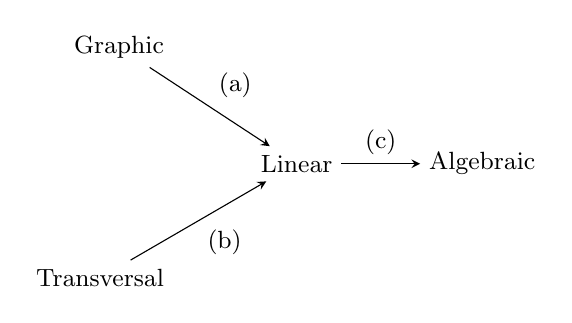
\begin{tikzpicture}\small
  \tikzset{>=stealth}
    \node (algebraic) {Algebraic};
    \node [left=of algebraic] (linear) {Linear}
    edge[->] node[above] {(c)} (algebraic) ;
    \node [above left=of linear] (graphic) {Graphic}
     edge[->] node[auto] {(a)} (linear);
     \node [below left=of linear] (transversal) {Transversal}
     edge[->] node[below right] {(b)} (linear);
  \end{tikzpicture}
\end{center}

\vspace{3pt}

We will start the proof by recalling the definitions given in class for linear, transversal, and graphical matroids.
We will define them by means of their ground set $\mathcal{E}$ and their independence sets $\mathcal{I}$.

\begin{definition}[Linear Matroid]
    Let $V$ be a vector space, then a linear matroid in $V$ is defined by
    \begin{equation*}
        \begin{split}
            \mathcal{E} & = \lbrace \text{ finite subset of } V \rbrace \\
            \mathcal{I} & = \lbrace \text{ linearly independent subsets of } \mathcal{E} \rbrace
        \end{split}
    \end{equation*}
\end{definition}

\begin{definition}[Graphical Matroid]
    Let $G = (V, E)$ be a graph,
    \begin{equation*}
        \begin{split}
            \mathcal{E} & = \lbrace \text{ edges of } G \rbrace = E \\
            \mathcal{I} & = \lbrace \text{ edges of forests of } \mathcal{G} \rbrace
        \end{split}
    \end{equation*}
\end{definition}

\begin{definition}[Transversal Matroid]
    Let $G = (U, V, E)$ be a bipartite graph,
    \begin{equation*}
        \begin{split}
            \mathcal{E} & = \lbrace \text{ bottom vertices of } G \rbrace = U \\
            \mathcal{I} & = \lbrace \text{ endpoints of maximal matchings } \mathcal{V} \rbrace
        \end{split}
    \end{equation*}
\end{definition}

To first prove (a), we want to build a linear matroid from a graphical one.
The first step is to choose our vector space, $U$.
Following the hint, let us define $U = \mathbb{R}^V$ whose standard basis is indexed by the vertices of $G = (V, E)$.
Then, if $V = \lbrace v_1, \dots, v_n \rbrace$ and $\lbrace e_{v_1}, \dots, e_{v_n}\rbrace$ is the standard basis in $U$, our ground and independence sets are defined as follows:
\begin{equation*}
    \begin{split}
        \mathcal{E} = \lbrace e_{v_i} - e_{v_j} : v_iv_j \in E \rbrace ;
        \hspace{5pt} \mathcal{I} = \bigcup_{f \text{ forest}} \lbrace e_{v_i} - e_{v_j} : v_iv_j \in E(f) \rbrace
    \end{split}
\end{equation*}
It just remains to prove that $\mathcal{I}$ as defined are indeed linearly independent subsets of $\mathcal{E}$.
Let's assume not, \textit{i.e.} one of such subset contains a linear dependence.
This is, for a forest $f$ in $G$ we have:
\begin{equation*}
    e_{v_k} - e_{v_l} = (e_{v_l} - e_{v_j}) + \dots + (e_{v_m} - e{v_n})
\end{equation*}
in this case it is clear that $k = n$ and there are two different paths to go from $v_l$ to $v_k$ what implies the existance of a cycle and hence $f$ is not a forest.
This contradicts our initial hypothesis and as a consequence $\mathcal{I}$ as defined is indeed an independence set what proves (a).

To prove (b) we will proceed in a similar manner.
In this case we have a bipartite graph $G = (E, F, H)$ where $E$ is the \textit{bottom} partition of vertices.
For our linear matroid we choose our vector space $V$ to be $\mathbbm{k}(X)^F$ with $\mathbbm{k}(X)$ defined as in the hint, and with standard basis indexed by vertices $f \in F$.
Then our ground, and independence sets are defined as follows:
\begin{equation*}
    \begin{split}
        \mathcal{E} = \left\lbrace \left\lbrace \sum_{f \in F, ef \in H} x_{e,f} u_f \right\rbrace : e \in E \right\rbrace ;
        \hspace{5pt} \mathcal{I} = \bigcup_{\text{$m$ max. matching}} \lbrace e : ef \in m, e \in E, F \in F \rbrace
    \end{split}
\end{equation*}
It just remains to prove that the sets in $\mathcal{I}$ are indeed independent.
In the same way we did for (a), we will assume some set not to be independent, hence yielding the following depndence relation:
\begin{equation*}
    \sum_{f \in F, e_1f \in H} x_{e_1,f} u_f = \sum_{f \in F, e_2f \in H} x_{e_2,f} u_f  + \dots + \sum_{f \in F, e_kf \in H} x_{e_1,f} u_f 
\end{equation*}
given that, by construction, the field extension $\mathbbm{k}(X)$ is defined by trascendentals $\lbrace x_{e,f}$, the equality can only hold iff some trascendental (\textit{e.g.} $x_{e_1,f}$ appears more than once, hence not being $m$ originally a matching in $G$.
This contradiction proves in turn (b).


\vspace{5pt}

\begin{center}
    \rule{5cm}{0.4pt}
\end{center}

\newpage

\textbf{\textit{(7) In each of the classes or models of matroids discussed in class (linear / graphical / transversal / algebraic matroids; hyperplane / affine hyperplane arrangements, matroid polytopes),}}

\hspace{5pt}\textbf{\textit{(a) describe independent sets, bases, circuits, cocircuits, and flats.}}

\vspace{3pt}

\begin{table}[]
\begin{tabular}{lllll}
                 & Linear                                                                                                                                     & Graphical                                 & Transversal       & Algebraic                                                                                                                         \\
Independent sets & Sets of linearly independent vectors                                                                                                       & Sets of edges that do not form any cycles & Matchings         & Sets of elements $\{\alpha_i\}$ that are algebraically independent and such that $\mathbb K[\{\alpha_i\}] \subset L$ is algebraic \\
Bases            & Bases (in the linear algebra sense)                                                                                                        & Spanning trees of a graph                 & Maximal matchings & Sets of elements $\{\alpha_i\}$ that are algebraically independent and such that $\mathbb K[\{\alpha_i\}] = L$                    \\
Circuits         & Sets ${v_1, \ldots, v_k\}$ such that $a_1 v_1 + \ldots + a_k v_k = 0$ for unique (up to multiplicative constant) $a_1, \ldots, a_k \neq 0$ (or, equivalent, such that no $k-1$ vectors out of the $k$ ones are on the same $k-2$-dimensional space & Simple cycles                             &                   &                                                                                                                                   \\
Cocircuits       &                                                                                                                                            &                                           &                   &                                                                                                                                   \\
Flats            & Sets of vector that generate all the vector space                                                                                          & Connected graphs                          & Maximal matchings & Sets of elements $\{\alpha_i\}$ such that $\mathbb K[\{\alpha_i\}] = L$                                                          
\end{tabular}
\end{table}
\vspace{3pt}

\hspace{5pt}\textbf{\textit{(b) For which of these entities can you rapidly see that they fulfill the corresponding axiom systems?  For which does it seem mysterious?.}}

\vspace{3pt}

WRITE HERE

\vspace{3pt}

\hspace{5pt}\textbf{\textit{(c) Describe the dual matroid of a matroid in each of these situations.}}

\vspace{3pt}

WRITE HERE


\vspace{5pt}

\begin{center}
    \rule{5cm}{0.4pt}
\end{center}

\newpage

\textbf{\textit{(8) We have seen that a matroid can be given by its collections of independent sets, bases, circuits, cocircuits, flats, or its rank function. Find algorithms to convert between as many of these entitites as you can. What is their combinatorial complexity?}}

\vspace{3pt}

For the rest of the exercise, it will be useful having the following graph in mind.
We will refer to specific algorithms by the letter of their edge.
In doing so, we won't assume anything on our ground set, neither on a theoretical implementation, we will just focus on the combinatorial complexity.
Note that we have chosen this \textit{bipartite} representation to improve readability.

\begin{center}
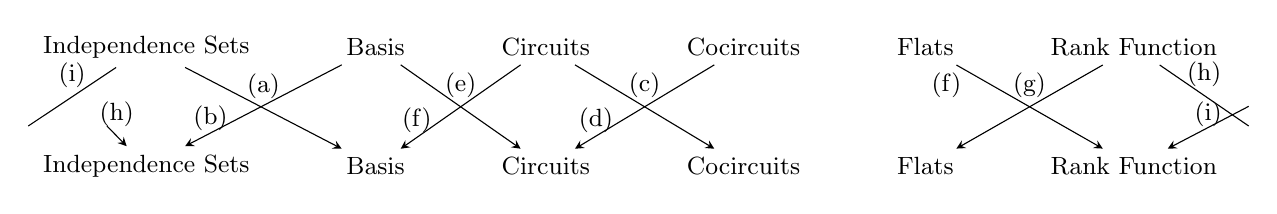
\begin{tikzpicture}\small
  \tikzset{>=stealth}
    % Top Row Nodes
    \node (independence-sets) {Independence Sets};
    \node [right=of independence-sets] (basis) {Basis};
    \node [right=of basis] (circuits) {Circuits};
    \node [right=of circuits] (cocircuits) {Cocircuits};
    \node [right=of cocircuits] (flats) {Flats};
    \node [right=of flats] (rank) {Rank Function};
    % Bottom Row Nodes
    \node [below=of independence-sets] (independence-sets-b) {Independence Sets};
    \node [right=of independence-sets-b] (basis-b) {Basis};
    \node [right=of basis-b] (circuits-b) {Circuits};
    \node [right=of circuits-b] (cocircuits-b) {Cocircuits};
    \node [right=of cocircuits-b] (flats-b) {Flats};
    \node [right=of flats-b] (rank-b) {Rank Function};
    \draw[->] (independence-sets) --  (basis-b) node[midway, above] {(a)};
    \draw[->] (basis) -- (independence-sets-b) node[near end, above, xshift = -5pt, yshift = -5pt] {(b)};
    \draw[->] (circuits) --  (cocircuits-b) node[midway, above] {(c)};
    \draw[->] (cocircuits) -- (circuits-b) node[near end, above, xshift = -5pt, yshift = -5pt] {(d)};
    \draw[->] (basis) --  (circuits-b) node[midway, above] {(e)};
    \draw[->] (circuits) -- (basis-b) node[near end, above, xshift = -5pt, yshift = -5pt] {(f)};
    \draw[->] (rank) --  (flats-b) node[midway, above] {(g)};
    \draw[-] (rank) --  (14,-1) node[midway, above] {(h)};
    \draw[->] (-0.5,-1) --  (independence-sets-b) node[midway, above] {(h)};
    \draw[-] (independence-sets) --  (-1.5,-1) node[midway, above] {(i)};
    \draw[->] (14,-0.75) --  (rank-b) node[midway, above, yshift=-3pt] {(i)};
    \draw[->] (flats) --  (rank-b) node[midway, above, xshift=-30pt, yshift=-0pt] {(f)};
  \end{tikzpicture}
\end{center}

Beneath we describe each algorithm indexed by the label of the edge and include its complexity:
\begin{itemize}
    \item[(a)] 
        We have that a set is independent if and only if it is a subset of a basis.
        In other words, a basis is a maximal independent set.
        To obtain $\B$ from $\I$ we iteratively, add independent elements to our basis with the caveat that subsets of already existing elements are discarded, and elements containing an already included one are swapped.
        The combinatorial complexity is $\mathcal{O}(|\I|^2)$.
    \item[(b)] Symmetrically, $\I$ is the power set of $\B$, from which the algorithm clearly follows. The complexity is ruled by printing or returning all elements in the set, which is $\mathcal{O}\left(\mathcal{P}(|\B|)\right)$.
    \item[(c)] Hull, B. \footnote{Hull, B. \textit{Two algorithms for Matroids}. Discrete Mathematics, Volume 13, Issue 2, 1975, Pages 121-128} presents an algorithm to, given the circuits of a matroid, find those of its dual matroid. The algorithm builds an element from $\C^*$ starting from one in $\C$ and using the elements of $E$. The algorithm in detail uses a recursion for which a more precise complexity calculation would be required. It is clear that, if we have the circuits of the dual matroid, we can find the cocircuits of the original one in linear time.
    \item[(d)] As proven in class, finding the dual of a matroid is linear in its size (doing Gauss, taking complements, ...). Further, given that the cocricuits are the circuits of the dual matroid, to obtain the cocircuits we can find the dual of the matroid (lineal time) and then apply (c).
    \item[(e)] A circuit is a minimally dependent set, all its proper subsets are independent. If we are given $\B$, we have to check whether adding a new element of $E$ creates a circuit or not. Note that, $\forall x \in E, \B \cup x$ contains one circuit but we want to make sure that it is minimally dependent. The algorithm consists then in for each $B \in \B = {x_1, \dots, x_b}$ and for each $x \in E$ we generate a circuit $C$ consisting of $x \cup \lbrace x_i : x_i \in B \wedge B \cup \{ x\} - x_i \in \B \rbrace$. The algorithm's complexity is then $\mathcal{O}\left(|\B||E||B|\right)$\footnote{E. Minieka, \textit{Finding the Circuits of a Matroid}. Journal of research of the National Bureau of Standards.}.
    \item[(f)] To obtain the basis of a matroid from its circuits, we have found a very intuitive and graphical algorithm presented by Hull in $1975^1$. In essence, it uses that no subset of a circuit is a circuit, and hence looks for a unique element in each circuit (it must exist) that makes it be minimally dependent. Removing it turns that circuit into a base. Looking for this odd elements (called \textit{pegs} in the original algorithm) can be done in linear time if implemented correctly. Then to find all basis we need to find all orderings of the induced basis from circuits. This last step rules our complexity.
    \item[(g)] This algorithm stems from the definition of a flat. A flat is a set whose closure is equal to itself, it is maximal in its rank. This is, adding an element would increase it's size. A naive algorithm would then be: for each subset  $S \subset E$, test the rank of $S \cup \{x \}$ for all $x \in E$ not in $S$. If every one adds to the current rank of $S$, then $S$ is a flat. The algorithm has complexity $\mathcal{O}(\mathcal{P}(E) \cdot |E|)$.
    \item[(h)] This algorithm also stems immediately from the fact that $A \subset E$ is an independence set iff it's rank equals its cardinality.
    \item[(i)] The rank function of a matroid, maps sets of elements to their rank. If a set $S \subset E$ belongs to $\I$, then it's rank will be its cardinality. Otherwise, the rank is the size of the maximum independence subset in $S$. A naive algorithm could be the following: for all $S \in E$, if $S \in \I$ we return $|S|$, otherwise, for each $U \in \I$ we look for that of maximum cardinality which is a subset of $S$. Hence, we can determine the rank of a set in $\mathcal{O}(|\I|)$.
    \item[(j)] We can implement a black-box style rank function using only the set of flats. To do so, we need to first know the maximum rank, $R$, of the sets of flats, $\F$. Then, given $S \subset E$, if $|S| = |E|$ we have its rank, which is maximum. Otherwise, we look for an element $F \in \F$ with only one element more, and compute the number of steps we take until we reach $E$. This number is the corank, which yields the corank. Alternatively, we could build the lattice of flats and compute this height manually.  
\end{itemize}

As a disclaimer and to finalize the exercise, we would like to note that we only present a subset of the algorithms we found.
Given the inherent (by definition) equivalences among many of the collections we defined, most algorithms could be easily rephrased to start from a different collection.
We have provided the sufficient selection to, concatenating one with the other, be able to get from any starting point to any ending point.


\vspace{5pt}

\begin{center}
    \rule{5cm}{0.4pt}
\end{center}

\end{document}
